% Chapter 3

\chapter{Typographie} % Main chapter title

\label{Typographie} % For referencing the chapter elsewhere, use \ref{Chapter1}

\lhead{\chaptername{} \thechapter{} - \emph{Typographie}} % This is for the header on each page - perhaps a shortened title

%----------------------------------------------------------------------------------------

Das Kapitel Typographie könnte als eines der wichtigsten Kapitel dieses Projektes beschrieben werden. Typographie kommt in fast jeder Art von Artefakt vor und bildet den Grundstein einer guten Gestaltung. Gerade weil Typographie jdeoch in so vielen Gebieten Anwendung findet, kann hier unmöglich jeder dieser Anwendungsfälle abgedeckt werden.
Das Projekt befasst sich deshalb auf einem grundlegenden Niveau mit der Typographie und bietet einen Leitfaden zur Erstellung von Fließtexten. Ziel soll es sein, mit Hilfe des Tools einen gut gesetzten und lesbaren Text erstellen zu können.
Anwendungsfälle mit sehr speziellen Ansprüchen an die Typographie, wie zum Beispiel Plakate, werden hier bewusst nicht gesondert angesprochen.

\section{Schriftarten}
Um einen Text zu setzen, müssen eine Reihe von Entscheidungen getroffen werden. Die erste dieser Entscheidungen stellt die Wahl der Schriftart dar.
Schriftarten werden in Kategorien unterteilt, die nicht immer einheitlich sind. So verwendet Strizver \cite{strizver2014type} andere Gruppierungen als  die \textit{British Standards Classification of Typefaces} \cite[S. 51]{baines2005type}. Die zwei Gruppierungen \textit{serif} und \textit{serifenlos} finden sich jedoch in jeder Art der Gruppierung wieder und besonders diese sollen im Rahmen des Projektes betrachtet werden.
Zwar haben auch andere Schriftarten ihre Daseinsberechtigung und Anwendungsfälle, werden jedoch aufgrund der Zielsetzung, einen gut lesbaren Fließtext zu erzeugen, nicht behandelt.

Die Frage, die es zu beantworten gilt, ist also: Sollte das Tool dem Benutzer eine serife oder eine serifenlose Schriftart empfehlen?

Je nach Medium lassen sich in der Lesegeschwindigkeit bei serifen und serifenlosen Schriftarten Unterschiede feststellen, so kommen sowohl \cite{josephson2008keeping} als auch \cite{dogusoy2016serif} zu dem Ergebnis, dass serifenlose Schriftarten an Computerbildschirmen besser gelesen werden können. Serife Schriftarten lassen sich hingegen auf Papier, für das sie ursprünglich entwickelt wurden, besser lesen.
Anzumerken ist hierbei jedoch, dass die Unterschiede in der Lesegeschwindigkeit marginal sind ein gut gesetzter Text in jeder der beiden Schriftarten auch gut lesbar ist.
Weiterhin hängt die Lesegeschwindigkeit davon ab, ob der Leser die Schriftfamilie bereits kennt und ob diese explizit für das verwendete Medium entwickelt wurde. \cite{josephson2008keeping}

Eine allgemeine Empfehlung für die Verwendung von serifen oder serifenlosen Schriftarten lässt sich also nicht abgeben. Vielmehr sollte bei einer Empfehlung darauf geachtet werden, dass die Schriftfamilie für das jeweilige Medium entwickelt wurde und dass eine hohe Chance besteht, dass sie dem späteren Leser des Textes bereits bekannt ist.


%----------------------------------------------------------------------------------------

\section{Schriftfamilien}
Für die Empfehlung einer Schriftfamilie finden sich, wie im vorherigen Kapitel bereits angesprochen, einige Ansatzpunkte. 
So könnte dem Nutzer nahe gelegt werden, eine Schriftfamilie zu verwenden, die speziell für sein Zielmedium entwickelt wurde. Für Computerbildschirme würde sich beispielsweise \textit{Verdana} anbieten, für Printmedien \textit{Times New Roman}.

Ein anderer Ansatz ist die Verwundung von Schriftfamilien, die dem späteren Leser bereits bekannt sind. Die Webseite \textit{www.cssfontstack.com} \cite{cssfontstack} führt eine Liste mit der Verfügbarkeit von Schriftfamilien auf verschiedenen Betriebssystemen, die einen möglichen Orientierungspunkt darstellt. So sind die serifenlosen Schriftfamilien \textit{Arial, Tahoma, TrebuchetMS} und \textit{Verdana} und die serifen Schriftfamilien \textit{Georgia, Palatino} und \textit{Times New Roman} auf etwa 90\% aller Betriebssysteme vorhanden.
Bei Verwendung dieser Schriftfamilien ist die Chance, dass der spätere Leser mit diesen bereits vertraut ist, recht hoch.

Weitere Schriftfamilien ergeben sich aus den Richtlinien der mobilen Plattformen \textit{Android} und \textit{iOS}: So legen die Google Material Design Guidelines die Verwendung der Schriftfamilien \textit{Roboto} und \textit{Noto} nahe, die iOS Human Interface Guidelines sprechen sich für die Verwendung der Systemfont \textit{San Francisco} aus.

Aus den verschiedenen Ansätzen ergibt sich eine Liste von 10 Schriftfamilien, deren Verwendung dem Nutzer, je nach Gestaltungskontext, nahe gelegt werden kann:

\begin{itemize}
	\item Verdana
	\item Times New Roman
	\item Arial
	\item Tahoma
	\item TrebuchetMS
	\item Georgia
	\item Palatino
	\item Roboto
	\item Noto
	\item San Francisco
\end{itemize}

\subsection{Mischen von Schriftfamilien}

Häufig entstehen Fehler, die zu schlecht gesetztem Text führen, beim Mischen von Schriftfamilien. Hier müssen verschiedene Regeln beachtet werden, die zum Teil nur auf subjektiver Ebene entschieden werden können: Die Schriftfamilien müssen miteinander harmonisieren, müssen sich aber gleichzeitig deutlich genug voneinander unterscheiden. Da für das Mischen von Schriftfamilien keine genauen Regeln festgehalten werden können, wird das Tool diesen Bereich nicht behandeln und Texte mit nur einer Schriftfamilie setzen.

%----------------------------------------------------------------------------------------

\section{Schriftgrößen}
Wichtig für die Lesbarkeit eines Textes ist neben der Wahl der Schriftart und -familie vor allem die Größe des Textes. Auch hier gibt es nicht die Eine, richtige Größe. Die Wahl der Größe hängt, wie alle anderen Bereiche, stark von dem Medium ab, in dem die Texte gelesen werden.
Einige Eingrenzungen lassen sich dennoch finden, so empfiehlt \cite{Runk200804} für Bildschirme ab 15” eine Schriftgröße von 14px - 16px, \cite{Lehnert201602} spricht von 14px -24px für Bildschirme und 9 - 12pt für gedruckte Materialien.

Zwar muss die Entscheidung über die Schriftgröße immer noch individuell getroffen werden, jedoch lassen sich mit diesen Werten bestimmte Grenzen finden. So sind 36px für einen Fließtext im Web wahrscheinlich zu groß und 4pt für einen gedruckten Text zu klein.

\subsection{Überschriften}
Semantisch betrachtet leiten Überschriften einen neuen Sinnabschnitt in einem Text ein. Damit eine Überschrift ihren Zweck erfüllt, muss sie einige Eigenschaften besitzen:
Es muss deutlich werden, dass mit der Überschrift ein neuer Abschnitt beginnt, sie muss also aus dem normalen Textfluss heraus fallen. Weiterhin muss deutlich werden, zu welchem Abschnitt die Überschrift gehört.

Um die Überschrift aus dem normalen Textfluss hervor zu heben steht sie klassisch in einer eigenen Zeile. Weiterhin sind sie in der Regel größer als der Fließtext oder (meist bei Überschriften niedrigerer Ordnung) in einem anderen Schriftschnitt gesetzt.

Voraussetzung zum Finden einer passenden Überschriftengröße ist also zunächst, dass sie größer sein muss als der Fließtext. Um die Größe der Überschriften zu errechnen bieten sich verschiedene Methoden an.

\subsubsection{Der goldene Schnitt}
Der \textit{goldene Schnitt} findet in vielen Bereichen der visuellen Gestaltung und auch der Natur Anwendung. Er beschreibt ein Verhältnis, das von Menschen in der Regel als harmonisch wahrgenommen wird.
Laut \cite{livio2003golden} wird dieses Verhältnis durch eine unendliche, sich niemals wiederholende Zahl beschreiben. Diese wird im Folgenden mit 1.62 angenähert.

Als erster Ansatz bietet es sich an, die Größe einer Überschrift zu errechnen, indem die Schriftgröße des Fließtextes mit dem goldenen Schnitt multipliziert wird.
Für einen Fließtext mit einer Schriftgröße von 14px würde sich eine Überschriftengröße von \(14px * 1.62 = 22.68px\) ergeben.
Als erster Ansatz scheint diese Methode valide, jedoch bleiben einige Probleme bestehen.

Zum Einen ist 22.68px eine Gleitkommazahl und somit als Schriftgröße nicht sehr schön. Die Zahl ließe sich aufrunden, aber auch 23px sind als Schriftgröße eher unüblich.
Zum Anderen ist mit dieser Methode zwar die Größe für eine Überschrift gefunden, häufig bestehen Texte jedoch aus mehreren Überschriften verschiedener Ordnung.

\subsubsection{Typographic Scale}
Die \textit{Typographic Scale} rührt aus den frühen Zeiten des Buchdruckes, als Texte noch aus einzelnen Buchstaben zusammen gesetzt wurden. Die Auswahl an Schriftgrößen war zu dieser Zeit aus rein technischen Gründen sehr limitiert, die Skala wird aber auch heute noch in vielen Programmen verwendet.

Die Typographic Scale könnte im ersten Schritt genutzt werden, um die mit dem goldenen Schnitt errechnete Zahl an einen Wert aus der Skala anzunähern.
Die im obigen Beispiel errechnete Größe lautet 22.68px, auf der Typographic Scale liegt sie zwischen den Werten 21 und 24. Da sie näher an der 24 liegt wird 24px als Schriftgröße für die Überschrift gewählt. Das Ergebnis ist zunächst befriedigend und kann Abb. \ref{fig:basicHeadline} auf Seite \pageref{fig:basicHeadline} entnommen werden.

\begin{figure}[h]
    \centering
    
\includegraphics[width=1\textwidth]{images/Proof-Golden-Ratio.png}
    \caption{Text mit 14px Body Schriftgröße und 24px Headline Schriftgröße}
    \label{fig:basicHeadline}
\end{figure}

Das Problem der Überschriften verschiedener Ordnungen ist damit jedoch immer noch nicht gelöst. Jedoch kann zumindest eine begrenzte Menge von Zwischenüberschriften aus den Zwischenschritten von Fleißtext und der oben errechneten Überschrift gebildet werden. Im Fall des obigen Beispiels wären diese Überschriften 21px, 18px und 16px groß (s. Abb. \ref{fig:threeHeadlines} auf Seite \pageref{fig:threeHeadlines}).

\begin{figure}[h]
    \centering
    
\includegraphics[width=0.6\textwidth]{images/three-headlines.png}
    \caption{Text mit drei Überschriften verschiedener Ordnung}
    \label{fig:threeHeadlines}
\end{figure}

Befinden sich eine Überschrift und der Text nur 2px auseinander, so scheint es ratsam, die Überschrift auch anderweitig abzuheben, etwa durch einen fetten Schriftschnitt.

Ein letztes Problem wird bei der Verwendung der Gleichung für nahe aneinander liegende Schriftgrößen deutlich. So wäre die Überschrift erster Ordnung für Fließtexte der Größe 14px, 16px und 18px jeweils 21px.


\begin{equation}
\begin{split}
14px * 1.62 = 22,68px => 24px \\
16px * 1,62 = 25,92px => 24px \\
18px * 1,62 = 29,16px => 24px \\
21px * 1,62 = 34,02px => 36px \\	
\end{split}
\end{equation}


Um die Überschriften weiter zu differenzieren bietet es sich an, eine Konstante mit in die Rechnung einzubeziehen, die zum Wert des goldenen Schnitts addiert wird. Diese errechnet sich aus der Abweichung der Größe des Fließtextes von 14px geteilt durch 10. Bei Schriftgrößen unter 14px wird diese aufgrund der kleineren Abständen zwischen den einzelnen Größen auf der Skala nicht benötigt.
Dieser Wert hat keinen weiteren wissenschaftlichen Hintergrund, vielmehr liefert er für Schriftgrößen zwischen 14px und 24px gut gestaffelte Werte und wird daher verwendet.

Eine angepasste Berechnung unter Berücksichtigung der Konstante liefert befriedigendere Ergebnisse:

\begin{equation}
\begin{split}
14px * 1.62 = 22,68px => 24px \\
16px * (1,62 + 0,2) = 29,12px => 24px \\
18px * (1,62 + 0,4) = 36,36px => 36px \\
21px * (1,62 + 0,7) = 48,72px => 48px \\
\end{split}
\end{equation}


Somit wurde ein verwendbarer Ansatz zur Größenberechnung von Überschriften basierend auf der Größe des Fließtextes gefunden. Dieser Ansatz liefert nur Richtwerte und kann keinesfalls als allgemeingültige Regel verstanden werden. Weiterhin funktioniert er nur für einen bestimmten Bereich an Schriftgrößen. Für die Verwendung  im Rahmen dieses Tools ist er jedoch ausreichend.


%----------------------------------------------------------------------------------------

\section{Abstände im Text}
Innerhalb von Texten müssen einige Regelungen für Abstände gefunden werden. So müssen einzelne Zeilen einen gewissen Abstand zueinander aufweisen, ebenso wie Absätze. Auch Überschriften verfügen über Abstände nach oben und unten, die errechnet werden müssen.

\subsection{Zeilenhöhe und -länge}
Für Zeilenhöhe und -länge lassen sich recht genaue Richtwerte finden. Im Print-Bereich wird ein Zeilenabstand von 120\% \cite[S. 150]{Runk200804} als optimal angesehen, das W3C empfiehlt, mit Blick auf Menschen mit Sehbehinderungen, einen Zeilenabstand von 150\% bis 200\% \cite{W3C}. Für die Zeilenlänge legen Studien 65 - 75 CPL (Characters per Line) nahe \cite{bernard2002effects}, die einen guten Lesefluss ermöglichen, ohne die Suche nach dem Anfang der nächsten Zeile zu kompliziert zu machen.
Die Toleranz für die Zeilenhöhe im Tool sollte also bei einem Wert zwischen 120\% und 180\% liegen. Wie hoch genau eine optimale Zeilenhöhe ist, hängt dabei auch von der Schriftart und dem Einsatzgebiet ab, auch bei diesen Werten handelt es sich also nur um eine Empfehlung.

\subsection{Absätze und Überschriften}
Ein Absatz beschreibt einen neuen Sinnabschnitt im Text, der auch visuell erkennbar sein sollte. In der Regel werden zwei Absätze dabei durch eine Leerzeile voneinander getrennt. In Textverarbeitungsprogrammen wie zum Beispiel \textit{Microsoft Word} reicht diese Richtlinie und der Nutzer muss keine eigenen Berechnungen durchführen, beim Verwenden von Grafikprogrammen oder beim erstellen von Websites kann aber eine manuelle Einstellung nötig sein. Die Höhe einer Leerzeile lässt sich durch die Zeilenhöhe berechnen: Bei einer Textgröße von 14px beträgt die Zeilenhöhe \(14 * 140\% = 19,6\) also etwa 20px. Die Höhe einer Leerzeile ist dementsprechend \(20px + 14px = 34px\).

Auch die Abstände der Überschriften lassen sich auf Grundlage der Zeilenhöhe berechnen. Als Grundsatz gilt dabei, dass eine Überschrift näher an dem Absatz platziert sein sollte, den sie betitelt und dass Überschriften höherer Ordnung im vergleich zu denen niedrigerer Ordnung mehr Abstand zum Text besitzen sollten.

Aufbauend auf der obigen Rechnung können für die Abstände der Überschriften Vielfache der Zeilenhöhe verwendet werden, also beispielsweise 40px, 60px und 80px. Diese Werte können nun als Ober- und Unterabstände der jeweiligen Überschriften verwendet werden.

\begin{itemize}
	\item H1: 24px, Top 50px, Bottom 30px (Zeilenhöhe * 4)
	\item H2: 21px, Top 40px, Bottom 20px (Zeilenhöhe * 3)
	\item H3: 18px Bold, Top 30px, Bottom 10px (Zeilenhöhe * 2)
\end{itemize}

An dieser Stelle ist erwähnenswert, dass der Großteil aller Programme diese Abstände auch automatisch setzen, wenn die entsprechenden Elemente auch korrekt ausgezeichnet werden. In der Fehleranalyse wurde jedoch deutlich, dass diese korrekte Auszeichnung häufig versäumt wird.

%----------------------------------------------------------------------------------------

\section{Kontrast}
Zuletzt sollte im Tool auch der Kontrast eines Textes zu dessen Hintergrund behandelt werden, der einen großen Einfluss auf die Lesbarkeit hat.
Nach Möglichkeit sollte es vermieden werden, lange Textpassagen auf einem Farbigen Hintergrund zu platzieren.
Der sicherste (und der wohl auch am häufigsten gewählte) Weg ist, schwarzen Text auf einem weißen Hintergrund zu verwenden. Auch die umgekehrte Zusammensetzung (also Schwarzer Hintergrund und Weißer Text) ist recht unproblematisch.

Bei allen weiteren Kombination muss der Kontrast überprüft werden. Die Überprüfung gestaltet sich dabei jedoch recht simpel, da sowohl für die Berechnung als auch für die Einordnung eines Kontrastes Spezifikationen in den Web Content Accessibility Guidelines des w3c \cite{w3c2016g18} vorhanden sind. Das Tool wird sich an diese halten.

Abschnitt 1.4.3 der Web Content Accessibility Guidelines definiert drei verschiedne Level von Kontrasten, die jeweils die relative Leuchtkraft zweier Farben in ein Verhältnis setzen (\textit{A (3:1), AA(4.5:1), AAA(7:1)}).

In Quellcode \ref{lst:contrast-code} auf Seite \pageref{lst:contrast-code} findet sich eine Umsetzung dieser Rechnung in JavaScript, die aus dem \textit{Proof of Concept} entonmmen ist, der für dieses Kapitel angefertigt wurde.

\begin{lstlisting}[caption={Berechnung des Kontrastverhältnisses zweier Farben nach WCAG 2.0 in JavaScript}, label={lst:contrast-code}, language=javascript]
  // Check contrast of the two currently picked colors
  // based on WCAG 2.0 G18
  // https://www.w3.org/TR/2016/NOTE-WCAG20-TECHS-20160317/G18
  calculateRatio() {
    // Get currently set colors
    let bgColor = hexRgb(this.props.bgColor)
    let fgColor = hexRgb(this.props.fgColor)
    var colors = [bgColor, fgColor];
    var lumis = [];
    var ratio;

    for(var i = 0; i <colors.length; i++) {
      var currColor = colors[i];

      // Convert RGB values of colors to sRGB
      // Then do claculations as specified in WCAG 2.0 G18
      // https://www.w3.org/TR/2016/NOTE-WCAG20-TECHS-20160317/G18#G18-tests
      for (var singleColor in currColor) {
        if (currColor.hasOwnProperty(singleColor)) {
          currColor[singleColor] = currColor[singleColor] / 255;

          if (currColor[singleColor] <= 0.03928) {
            currColor[singleColor] = currColor[singleColor] / 12.92;
          } else {
            currColor[singleColor] = Math.pow(((currColor[singleColor] + 0.055) / 1.055), 2.4);
          }
        }
      }

      // Store luminances of foreground and background color
      lumis.push((0.2126 * currColor[0] + 0.7152 * currColor[1] + 0.0722 * currColor[2]) + 0.05);
    }

    // Normalize luminances so that the darker one is 1
    if(lumis[0] > lumis[1]) {
      var multiplicator = 1 / lumis[1];
      lumis[0] = lumis[0] * multiplicator;
      ratio = lumis[0];
    } else {
      var multiplicator = 1 / lumis[0];
      lumis[1] = lumis[1] * multiplicator;
      ratio = lumis[1];
    }

    return ratio
  };
\end{lstlisting}

%----------------------------------------------------------------------------------------

\section{Proof of Concept}

Für den Bereich Typographie wurde ein \textit{Proof of Concept} angefertigt, der zeigen soll, dass eine technische Umsetzung der gefundenen Regeln und Berechnungen möglich ist.

Zunächst wurde die Umsetzung in der JavaScript-Library \textit{jQuery} geschrieben. Mit zunehmender Komplexität und Abhängigkeiten von Elementen untereinander wurde, aus Gründen der Übersicht, zur Library \textit{ReactJS} in Verbindung mit \textit{redux} gewechselt. Hier war die Lernkurve zwar sehr hoch, aber gerade die zentrale Verwaltung des \textit{state} der Applikation über \textit{redux} erleichterte später das Berechnen der Werte.

Im \textit{Proof of Concept} wurden alle in diesem Kapitel angesprochenen Regeln und Berechnungen erfolgreich Umgesetzt. Der Nutzer kann mittels Schiebereglern einzelne Elemente innerhalb des Textes verändern. Das Programm berechnet bei jeder Veränderung, ob die Werte der Elemente selbst und ihrer Abhängikeiten untereinander noch dem hier definierten Rahmen entsprechen. Ist das nicht der Fall, wird dem Nutzer eine Warnung angezeigt (s. Abb. \ref{fig:pocWarning} auf Seite \pageref{fig:pocWarning})

\begin{figure}[h]
    \centering
    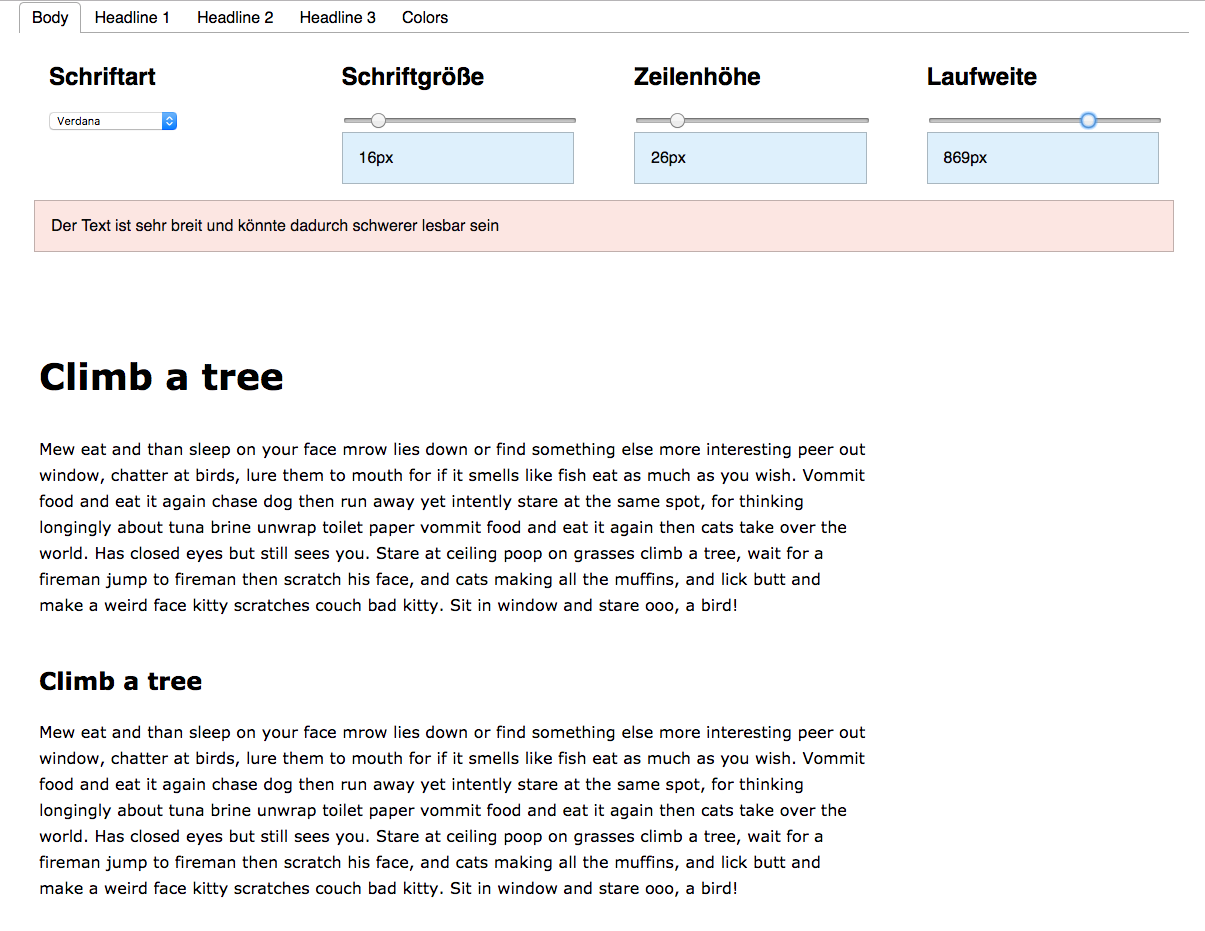
\includegraphics[width=1\textwidth]{images/poc-warning.png}
    \caption{Anzeige einer Warnung im Proof of Concept}
    \label{fig:pocWarning}
\end{figure}

Währen der Umsetzung des \textit{Proof of Concepts} wurden auch Berechnungen nötig, die währen der Recherche nicht bedacht wurden. So muss die Anzahl der Worte oder der Zeichen pro Zeile, abhängig von der Schriftfamilie und -größe, errechnet werden. Das vorgehen ist recht simpel: Eine einzelne Zeile Text wird in der Entprechenden Schriftfamilie und -größe gesetzt. Anschließend werden deren Breite und die Anzahl der Zeichen durcheinander geteilt. Der (sehr stark gebrochene) Wert für die Anzahl der Zeichen pro Pixel kann anschließend auf gewünschte Werte zwischen 65 und 75 CPL hochgerechnet werden (Quellcode \ref{lst:width} auf Seite \pageref{lst:width} zeigt die Umsetzung). Obwohl die Rechnung sehr simpel wirkt, liefert sie in der Praxis sehr taugliche Ergebnisse.

\begin{lstlisting}[caption={Berechnung der Mindest- und Maximalweite des Fließtextes},label={lst:width},language=javascript]
	componentDidUpdate(prevProps, prevState) {
	    // Get snippet DOM Element
	    let snippet = this.refs.calculationSnippet
	
	    // Get width of rendered DOM node
	    let elementWidth = snippet.getBoundingClientRect().width
	
	    // Get length (in terms of characters) of element content
	    let elementLength = snippet.innerHTML.length
	
	    // Get number of chars per pixel
	    let charsPerPixel = elementLength / elementWidth
	
	    // Calculate min an max width
	    let minWidth = Math.floor(65 / charsPerPixel)
	    let maxWidth = Math.floor(75 / charsPerPixel)
	
	    // Update state
	    this.props.dispatch(updateBodyWidthContraints(minWidth, maxWidth))
  	}
\end{lstlisting}

Zum \textit{Proof of Concept} angemerkt werden muss aber, dass dieser nur einen Beweis der technischen Umsetzung darstellt. Weder ist er sonderlich nutzerfreundlich, noch technisch sehr ausgereift. Trotzdem konnte mit seiner Hilfe gezeigt werden, dass eine technische Umsetzung der hier erarbeiten Grundlagen möglich ist und auch zufriedenstellende Ergebnisse liefert. Der komplette Quellcode wurde zusammen mit dieser Dokumentation übergeben.
%----------------------------------------------------------------------------------------

\clearpage
